% main.tex
%
% This file groups together all of the chapters, which are stored as neighboring files in this
% directory. It also establishes the general formatting of the paper, as specified here:
%   https://www.cs.ox.ac.uk/teaching/courses/projects/handbook/Project%20Handbook%202021.pdf
% And finally, it defines a number of commands that are used elsewhere.

\documentclass[12pt]{article}
\usepackage[paper=a4paper,margin=3cm]{geometry}
\frenchspacing

\usepackage[utf8]{inputenc}

\usepackage{amsmath}
\usepackage[toc]{appendix}
\usepackage{bm}
\usepackage[font=small,labelfont=bf]{caption}
\usepackage{changepage}
\usepackage{float}
\usepackage[splitrule]{footmisc}
\usepackage{graphicx}
\usepackage{hyperref}
\usepackage{mhchem}
\usepackage{multirow}
\usepackage[square,numbers]{natbib}
\usepackage{pgfplots}
\usepackage{subcaption}
\usepackage{textcomp}
\usepackage{titlesec}
\usepackage{tikz}
\usetikzlibrary{decorations.pathreplacing}
\usetikzlibrary{calc}
\usepackage{xcolor}

% funky helper stuff taken from https://tex.stackexchange.com/a/172095
% helps with braces in figs/bifurcation.tikz.tex
\makeatletter
\pgfdeclaremetadecoration{tikz@internal}{pre}{
  \state{pre}[width=\pgfkeysvalueof{/pgf/decoration/pre length}, next state=main]
  {
    \tikz@dec@trans
    \decoration{\pgfkeysvalueof{/pgf/decoration/pre}}
  }
  \state{main}[width=\pgfmetadecoratedremainingdistance-\pgfkeysvalueof{/pgf/decoration/post length}, next state=final]
  {
    \tikz@dec@trans
    \decoration{\tikz@decoration@name}
  }
  \state{final}
  {
    \tikz@dec@trans
    \decoration{\pgfkeysvalueof{/pgf/decoration/post}}
  }
}
\makeatother

% never break footnotes across pages -- https://tex.stackexchange.com/a/32210
%
% ... although this doesn't seem to be working as effectively as it should.
\interfootnotelinepenalty=10000

% A selection of colors making up a pastel-like palette, just so everything's a bit more pleasing on
% the eye.
\definecolor{softgrey}{HTML}{808080}
\definecolor{softblue}{HTML}{4C70D4}
\definecolor{softgreen}{HTML}{26AB56}
\definecolor{softyellow}{HTML}{EBE426}
\definecolor{softorange}{HTML}{F57E16}
\definecolor{softred}{HTML}{CF463C}

% Used as an "almost" `softblue`
\definecolor{softsoftblue}{HTML}{698DF0}

% Usage: \code{ <text> }
%
% Produces inline code formatting.
\newcommand{\code}[1]{\texttt{#1}}

% Usage: \breakpars
%
% Adds a little bit of space in between paragraphs.
\newcommand{\breakpars}{\vspace{0.1in}}

% Usage \norm { math mode content }
%
% Outputs the norm / magnitude / absolute value of the contents - || contents ||
% Taken from https://tex.stackexchange.com/a/107190
\newcommand{\norm}[1]{\left\lVert#1\right\rVert}

% Usage \tightbox { content, e.g. \includegraphics{..} }
%
% Creates a box that exactly borders the content
\newcommand{\tightbox}[1]{%
    {\setlength{\fboxsep}{0pt}\fbox{#1}}%
}

% \newcommand{\todo}[1]{%
%     \begin{adjustwidth}{-0.5cm}{-0.5cm}{%
%         \noindent\textcolor{red}{Todo:} \bf{#1}%
%     }\end{adjustwidth}%
% }

\begin{document}

% Title page

\begin{titlepage}
\begin{center}
    \Huge
    \textbf{Investigations using a virtual lung model}
    
    \vspace{1.5cm}
    \textbf{Max Sharnoff}
    
    Trinity 2022 \\
    BA Computer Science
\end{center}
\end{titlepage}

% Blank page
\newpage\ \addtocounter{page}{-1} \thispagestyle{empty}

% Abstract
\newpage
% Abstract.tex
%
% vim: set ft=tex:

{\Large \textbf{Abstract}}

\vspace{0.5cm}

Detecting changes in human lung morphology and determining its effects on lung function requires
significant time committment per patient, so statistical analysis on many individuals is infeasible.
Computational models of the lung are therefore a natural choice for researching the effects of
altered lung morphology, with reference to existing lung function tests.

Accurate computational models also allow investigation into properties of the lungs that cannot
feasibly be measured; e.g., increased internal stress in one location from damaged airways
elsewhere.

This paper builds on recent advancements in modelling airflow in the lungs (e.g.,
\cite{FoyEtAl2017}) to create a tool for efficient, accurate computational models of the lungs that
supports mid-simulation alterations to lung morphology. We use a fraction of the capabilities of
this tool to investigate the effects of whole and partial-lung constriction.


% Table of contents
\newpage
\tableofcontents

\newpage
% Ch1-introduction.tex
\section{Introduction}

General ideas: \\
Full fluid dynamics simulations of the lungs is difficult. Thankfully, we don't need that. We can
get pretty accurate results by building on Brody's work, simulating airflow as 1D and
incompressible.

Using this model allows us to model how the airflow changes under a number of conditions, e.g.
damage to the alveoli in a region, constricting bronchioles, etc.


\newpage
% Ch2-background.tex
\section{Background}



\newpage
% Ch3-methods.tex
%
% vim: set ft=tex:
\section{Methods}

This section is mostly some temporary filler at the moment, just serving as a place to jot down the
formulae that we're using inside the simulation \textit{right now}.

\subsection{Simultaneous Equations}

There are essentially four simultaneous equations that we use to evaluate the state of the system at
a given point in time. This section provides a summary and brief description of each, the first of
which is the following:

\begin{equation}
    P_{\text{parent}(i)} - P_i = R(i) Q_i
\end{equation}

\noindent
which specifies that the pressure differential between the distal end of branch $i$ and its parent
must equal the pressure from the resistance from the flow through this branch $i$. For the ``root''
branch, $P_{\text{parent}(i)}$ is the pressure at the trachea~--~typically atmospheric pressure.

The resistance term $R(i)$ is defined as following function, as given by Pedley et al. (1970):

\begin{equation*}
    R(i) = \frac{2 \mu L_i c}{\pi r_i^4} \left( \frac{4 \rho |Q_i|}{\mu \pi L_i} \right)^{\frac{1}{2}}
\end{equation*}

The parenthesized term corresponds to the Reynold's number of the flow, scaled by the ratio of the
diameter of the branch to its length $L_i$. $r_i$ is the radius of branch $i$, $\mu$ is the
viscosity of the air, and $c = 1.85$ is a correction constant.

The second equation ensures incompressibility; the flow through a bifurcation must equal the sum of
the flow through its children:

\begin{equation}
    Q_i = \sum Q_{\text{child}}
\end{equation}

\noindent
where each \textit{child} refers to any branch $c$ with $\text{parent}(c) = i$.

The third equation maintains that the volume of an acinar region changes with the flow into or out
of it for the given timestep:

\begin{equation}
    V_i^t = V_i^{t-1} + dt Q_i^t
\end{equation}

\noindent
where $dt$ is the timestep size, $t$ refers to the current timestep, and $V_i$ is the volume of the
acinar region of branch $i$.

The final equation defines the elastic force of each acinar region, relating the pressure it exerts
on its branch to the volume of the region itself and the pressure outside it:

\begin{equation} \label{eq:acinar-pressure-volume-naive}
    P_i = \frac{1}{C_i} V_i + P_{pl}(t)
\end{equation}

\noindent
where $P_{pl}(t)$ is the pleural pressure (i.e. the ``pressure'' from the diaphragm, outside the
acinar region) at the current time and $C_i$ is the \textit{compliance} of the acinar region of
branch $i$. The pleural pressure changes over time to mimic human breathing patterns~--~hence why it
is parameterised by $t$.

\breakpars

At each timestep in the simulation, all of the simultaneous equations are grouped into a single
optimization function $f(\bm{x}) = (\text{EQ}_1..., \text{EQ}_2..., \text{EQ}_3..., \text{EQ}_4)$,
where each $\text{EQ}_i$ corresponds to the repeated instances of the $i$th equation above,
normalized so the right-hand-side equals zero. Thus the solution exists at $\bm{0}$, and we use
Euler's method to find an approximate solution, within $\norm{f(\bm{x})}^2 \le tol$ and
$\norm{dx}^2 \le tol$, with a tolerance of $10^{-6}$.

The input $\bm{x}$ is arranged with the values $(P..., Q..., V...)$ for each applicable
branch~--~i.e. using $P$ and $Q$ from all branches and $V$ from each acinar region.

\breakpars

The above descriptions are \textit{nearly} correct~--~they would work, but there were a few
adjustments made to the inputs and equations in practice for better numerical stability. These are
discussed in the \hyperref[sec:units-and-numerical-stability]{next section}.

\subsection{Units \& Numerical stability} \label{sec:units-and-numerical-stability}

It is worth making explict the units used for each value. After careful consideration, these were
considered to provide the best trade-off of familiar units and those with values of magnitude close
to one, where floating-point accuracy is maximized. As we will see momentarily, the spread was still
quite wide. The chosen units were:

{
    % Add a bit more spacing within the rows of the table
    \renewcommand{\arraystretch}{1.6}
    \begin{table}[h]
    \centering
    \begin{tabular}{ |c|c| }
        \hline
        Type of thing ??? & Units \\
        \hline \hline
        Distance & $\text{m}$ \\
        \hline
        Volume & $\text{m}^3$ \\
        \hline
        Flow velocity & $\frac{ \text{m}^3 }{ \text{s} }$ \\
        \hline
        Density & $\frac{ \text{kg} }{ \text{m}^3 }$ \\
        \hline
        Pressure & Pascals $\left( \frac{ \text{kg} }{ \text{m} \cdot \text{s}^2 } \right)$ \\
        \hline
        Compliance & $\frac{ \text{m}^3 }{ \text{Pascal} }$ $\left( \frac{ \text{m}^4 \cdot \text{s}^2 }{ \text{kg} } \right)$ \\
        \hline
        Resistance & $\frac{ \text{kg} }{ \text{m}^4 \cdot \text{s} }$ \\
        \hline
        Viscosity & $\frac{ \text{kg} }{ \text{m} \cdot \text{s} }$ \\
        \hline
    \end{tabular}
    \end{table}
}

One of the challenges with using these units is that some values are at a much greater magnitude
than the others. For example, the pressure inside each branch is close to atmospheric pressure~--~or
about $10^5$ Pascals, but pressure \textit{gradients} are typically much smaller.

In practice, this can mean that if the $dx$ from our Euler step is too small, the pressure won't
change; it doesn't have the necessary precision at that magnitude.

\breakpars

To mitigate this issue, we define two new values: $\hat{P}$ and $\hat{V}$, which are given by:

\begin{equation}
    \hat{P} = P - P_{\text{atm}}
\end{equation}

\noindent
where $P_{\text{atm}}$ is is atmospheric pressure; and:

\begin{align}
    \hat{V} & = V - V \vert_{P = P_{\text{atm}}} \\
            & = C (\hat{P} - P_{pl})
\end{align}

\noindent
Note that the definition of $\hat{V}$ would be the result of simply substituting $\hat{P}$ for $P$
in \ref{eq:acinar-pressure-volume-naive}. Applying these substitutions gives the following
equations, equivalent to their counterparts above:

\begin{equation}
    \hat{P}_{\text{parent}} - \hat{P}_i = R(i) Q_i
\end{equation}

\begin{equation}
    Q_i = \sum Q_{\text{child}}
\end{equation}

\begin{equation}
    \hat{V}_i^t = \hat{V}_i^{t-1} + dt Q_i^t
\end{equation}

\begin{equation}
    \hat{P}_i = \frac{1}{C_i} \hat{V}_i + P_{pl}(t)
\end{equation}

Representing the pressure and volume by their \textit{offset} from values at atmospheric pressure
causes them to cluster much closer to zero~--~the magnitude of the mean is significantly decreased,
relative to the variance of the values. This of course greatly improves the accuracy of each Euler
step.


\newpage
% Ch4-results.tex
%
% vim: set ft=tex:
\section{Results} \label{sec:results}

Before properly describing the results, it is worth providing some context for the typical
parameters used for running the various simulations. Unless otherwise indicated, we use the
following values: approximate FRC of 3 L, trachea length of 10 cm, trachea radius of 0.95 cm,
pleural pressure range from $-875$ to $-750$ Pa with a period of 4 seconds, bronchiole length
decrease of 27\% per generation, bronchiole radius decrease by 23\% per generation, and a depth of
10 generations (i.e. 512 acinar regions). The depth was limited by the computational resources
required to simulate hundreds of different models.

Values for the trachea are taken as a middle-ground from \autoref{tab:lung-sizes} and bronchiole
size decrease is derived so that the same fractional decrease per generation results in the
appropriate sizes at transitional bronchioles (also from \autoref{tab:lung-sizes}). The pleural
pressure is adapted from \cite{BenTal2006}, using an idealized model of elasticity for an
approximate tidal volume of 0.5 litres.

We typically use a timestep of 0.01s for the simulation, with smaller timesteps sometimes used to
get higher-fidelity output (e.g., for \autoref{fig:constricted-flow-stats}).

\subsection{Observed numerical stability}

\begin{figure}[ht!]
    \centering
    \begin{tikzpicture}[scale=0.8]
        \input{figs/initial-volumes-level-out.generated.tex}
        \input{figs/initial-volumes-too-constricted.generated.tex}
    \end{tikzpicture}
    \caption{
        Simulated volume at the start of a breathing cycle, with varied initial volumes. Both
        experiments with a symmetric model with a depth of 10 generations. Graphs display the
        distinction between unrestricted (left) vs 40\% constricted (right). \textbf{Note:}
        displayed timespan differs between the left and right graphs.
    }
    \label{fig:different-initial-volumes}
\end{figure}

To be confident in the results of other experiments, it is first crucial to determine that the
simulation remains stable after running for extended periods of time. To do this, we simulated a
simpler model (fully symmetric, no constriction, depth of 10) for 1000 seconds~--~which required
100,000 simulation ticks.

It is at this point that we'd ideally reference some figure to show that the system is stable in
this configuration, but the series of volumes at each timestamp~--~starting at 4, 100, and 1000
seconds~--~were all the same, up to nine significant figures. By the end of the first breath cycle,
the volume had corrected from the starting volume of 3 to 3.019 litres. Total volume of air in the
lungs over the course of each ``breath'' did not change over the course of an atypically lengthy
experiment, indicating a high degree of numerical stability (as expected, due to our use of an
implicit Euler method).

\breakpars

We also considered that the initial volume used in experimentation is not guaranteed to be accurate
to the ``typical'' volume at that point in the breathing cycle~--~a fact that becomes visible with
higher degrees of airway constriction (discussed in \autoref{sec:flow-characteristics}). Therefore,
we also experimented with significantly changed initial volumes, as shown above in
\autoref{fig:different-initial-volumes}. The system quickly recovers from pertubations when airflow
is unrestricted, but is slower to return to the typical volume when resistance prevents the
correction from being made more quickly.

\subsection{Flow characteristics under stable constriction} \label{sec:flow-characteristics}

\begin{figure}[ht!]
    \centering
    \begin{tikzpicture}
        \input{figs/constricted-flow-characteristics.generated.tex}
    \end{tikzpicture}
    \caption{
        Stable flow during two breathing cycles with varied levels of whole-lung airway
        constriction. Measurements were only recorded after 20 seconds to ensure the effects of any
        starting conditions had been minimized, shown necessary at severe constriction by
        \autoref{fig:different-initial-volumes}.
    }
    \label{fig:constricted-flow-characteristics}
\end{figure}

The first set of experiments investigated the behavior of sustained, normal breathing under minimal
to severe constriction. Here, we used whole-lung constriction~--~limiting the radius of all airways
by a given fraction. \autoref{fig:constricted-flow-characteristics} displays the recorded airflow at
the larynx for normal breathing under a few different levels of constriction. The function
determining pleural pressure was kept constant.

As constriction increases, there are three visible effects: the maximum flow decreases, the time of
the peak in flow shifts later, and the shape of the flow curve also changes~--~becoming flatter at
its peaks and troughs and steeper around the transitions between positive and negative flow.

\autoref{fig:constricted-flow-stats} quantifies these effects, with additional data provided for
dilation of the airways. Our analysis here includes the range of airway widths covered by dilation
because it provides information that may correspond to humans with naturally wider airways.

Maximum flow slowly decreases from 50\% dilation to none, after which it curves more steeply towards
zero. However, before the \textit{amount} of flow changes significantly, the effects of constriction
are readily visible in other characteristics of the curve~--~particularly the maximum acceleration:
it increases from 50\% dilation to around 10\% constriction, at which point its magnitude starts to
become limited by the height of the flow curve.

\begin{figure}[ht!]
    \centering
    \begin{subfigure}[t]{.45\textwidth}
        \centering
        \begin{tikzpicture}[scale=.75]
            \input{figs/constricted-flow-stats-maxflow.generated.tex}
        \end{tikzpicture}
        \subcaption{
            Maximum flow and time it occurs relative to no constriction
        }
    \end{subfigure}%
    \hspace{2em}%
    \begin{subfigure}[t]{.45\textwidth}
        \centering
        \begin{tikzpicture}[scale=.75]
            \input{figs/constricted-flow-stats-acceleration.generated.tex}
        \end{tikzpicture}
        \subcaption{
            Maximum flow and maximum acceleration in flow
        }
    \end{subfigure}%
    \caption{
        Changes in airflow characteristics as constriction increases from dilation by 50\% to 90\%
        constriction. Peak airflow is displayed as a baseline for both the time maximum flow occurs
        (left) and the maximum acceleration in flow between simulation ticks (right).
    }
    \label{fig:constricted-flow-stats}
\end{figure}

Some uneveness is present in the graph of maximum aceleration. Initially, this was thought to be due
to the particular way that it is being measured, namely: finding the greatest increase in flow from
one simulation tick to the next. Slight differences in the timing could have meant that the maximal
acceleration had some local variability despite the global trend.

To test this, we ran the simulation with a timestep of 1/400s instead of the usual 1/100s, the
results of which are in \autoref{fig:constricted-flow-stats}. The peak is much greater (up from
approx. 2 L/s\textsuperscript{2} to approx. 3.5), indicating that there was a degree of the most
extreme points not being captured. This may still be the case, even at 1/400s~--~as improbable as it
seems.

\subsection{Recovery}

\begin{figure}[ht!]
    \centering
    \begin{tikzpicture}[scale=0.6]
        \input{figs/recovery-healthy.generated.tex}
        \input{figs/recovery.generated.tex}
        \input{figs/recovery-constricted.generated.tex}
    \end{tikzpicture}
    \caption{
        Side-by-side comparison between unconstricted flow (left), gradual constriction and recovery
        (middle), and constricted flow (right). The target constriction level was 50\%, with
        \code{tanh} used for interpolation. For the recovery, transitions between constriction
        levels were 4 seconds each, onset was at 8 seconds, and recovery started at 16 seconds.
    }
    \label{fig:demo-recovery}
\end{figure}

Using the scheduled constriction feature of the software made for this project, we ran a number of
trials that started with a ``healthy'' lung, then slowly constricted the airways to a target
constriction (smoothing with interpolation functions from \autoref{sec:interpolation}), stayed
constricted for a full breath, and then gradually reduced constriction back to the healthy state.

An example of this is given in \autoref{fig:demo-recovery}, with baseline comparisons for the flow
and volume of the lung under no constriction or the target of constriction by 50\%. All three models
were run for 4 seconds at the start to even out any disturbances from the initial state. At 8
seconds, the recovery trial starts to constrict, but it only starts to become noticeable at around
11 seconds (discounting the raised trough at 9 seconds)~--~before finally reaching the target
constriction at 12 seconds. From there, the flow appears nearly identical to the constricted
baseline, with a slightly higher than baseline flow briefly at the 12 second mark. In a similar
fashion, recovery starts after a full breath cycle, at 16 seconds. The effects of reducing
constriction are almost immediately visible, with an unusually sharp increase in flow at 18 seconds.
At 20 seconds, the constriction has been fully removed and flow appears normal.

\breakpars

There is a lot of information in the above paragraph~--~to summarize briefly: the most visible
effect in this trial of changing constriction levels is that volume and flow tends to quickly match
the characteristics that we would expect from the constriction level it reaches. Some atypical
behavior \textit{is} observed around these transitions, but it is brief (e.g., the flow at 18s).

To demonstrate the causes behind this atypicality, \autoref{fig:demo-recovery-matched} overlays the
recovery and baseline trials with a sort of ``matched baseline``~--~composite curves made by taking
from the baseline curve matching the constriction level each datapoint. For example: at 10 seconds,
the model is constricted by 25\%, so the ``matched baseline'' at 10 seconds uses the flow and volume
from a steady run at 25\% constriction at 10 seconds.

\begin{figure}[tp]
    \centering
    \begin{tikzpicture}
        \input{figs/recovery-matched.generated.tex}
    \end{tikzpicture}
    \caption{
        The same recovery trials from \autoref{fig:demo-recovery}, compared with the values of
        volume and flow corresponding to a stable breath pattern at the current constriction level,
        at each point in time (``Matched''). Much of the jaggedness is due to the imprecision in
        linearly interpolating between the two closest constriction trials (to the nearest integer
        percentage).
    }
    \label{fig:demo-recovery-matched}
\end{figure}

Looking at \autoref{fig:demo-recovery-matched}, it's tempting to think that the recovery trial
directly follows the matched baseline. However, while changing the constriction level (i.e. airway
raidii), the only variable that remains different between trials is the volume; everything else is
derived from the airway morphology and pleural pressure, the latter of which we have kept
consistent. The simulation has no ``knowledge'' of the appropriate volume to correct to.

Instead, the matching \textit{must} be a direct result of the way that the flow due to the current
volume and pleural pressure is limited (or allowed) by the airway widths. With greater constriction,
the flow becomes more limited by resistance from smaller airways, which is why we see a reduced
tidal volume, even though the compliance and pleural pressure haven't changed.

When recovery is introduced, this effect tends to \textit{imitate} the matched baseline, but only
where the volume is already similar~--~and changes in volume are limited by airway resistance. This
is most visible in the way that the recovery trial stays distinctly separate from the constricted
baseline for most of the period in which it is at that constriction level: the initial raised volume
takes time to correct for.

The effects at 18-19 seconds are similar in nature: the recovery trial initially diverges from the
matched baseline because its volume at, e.g., 17.5 seconds is less than would be expected for the
level of constriction at 18 seconds. Because of this difference, the recovery trial maintains inward
flow for longer as the pleural pressure starts to increase. Eventually at 18.5s, the slowed upward
trend in volume meets the matched baseline and snaps to the same flow~--~because the volume and
pleural pressure are the same.

\subsubsection{Generalizing recovery}

All of the above serves to illustrate some of the ways in which flow can be disrupted by actively
changing the level of whole-lung constriction. There are a couple of general findings to note.

Firstly: airway size matters, both ``healthy'' and constricted. In our early experimentation, we
found that unusually wide airways~--~precisely because they have so little resistance~--~can easily
result in large spikes in airflow as out-of-phase constricted volume is adjusted with loosening
constriction and large negative pleural pressure.

Secondly, the precise nature of the abnormal flow that we see when recovering from constricted
airways varies greatly depending on the timing (relative to each breath) and speed of the recovery.
This can similarly be selected to produce similar effects as above, as demonstrated in
\autoref{fig:sharp-recovery}. Abnormally high flows can be created from normal pressures simply by
forcing the volume to remain mostly constant as the pleural pressure changes beneath it. This is
essentially akin to breathing in, closing the epiglottis, fully relaxing the diaphragm, and then
opening the epiglottis~--~releasing the air quicker than would normally happen as the diaphragm
slowly relaxes.\footnotemark

\footnotetext{
    In practice, this demonstration tends not to be very extreme (due to the diaphragm moving slowly
    even when relaxed). A more sudden example is the reverse: contracting the diaphragm without
    breathing in, then allowing air to enter the lungs.
}

\begin{figure}[hb]
    \centering
    \begin{tikzpicture}
        \input{figs/sharp-recovery.generated.tex}
    \end{tikzpicture}
    \caption{
        Extreme example of timed severe constriction (by 80\%) causing large spikes in flow.
        Constriction begins at 6.1s, takes full effect within 0.1s, and starts returning to normal
        at 7.7s, also taking 0.1s.
    }
    \label{fig:sharp-recovery}
\end{figure}

Of course, the type of breathing shown in \autoref{fig:sharp-recovery} is highly unlikely to happen
in practice~--~primarily because real humans will tend to react to their internal lung state by
indirectly changing the pleural pressure in a way that our model cannot. This is discussed in more
detail in \autoref{sec:limitations-and-further-work}.

\subsection{Asymmetric constriction}

\begin{figure}[h]
    \centering
    \begin{tikzpicture}
        \input{figs/asymmetric.generated.tex}
    \end{tikzpicture}
    \caption{
        Asymmetric constriction and recovery, with onset of left lung constriction at 8s, reaching
        the final 50\% constriction by 12s via \code{tanh} interpolation, and recovering from
        16-20s.
    }
    \label{fig:asymmetric-recovery}
\end{figure}

The final experiment performed was around the use of asymmetric constriction. We ran the same trial
as from \autoref{fig:demo-recovery-matched}, but limited the constriction to just the left side of
the lung. The separate volume and flow between the two equal halves are paired in
\autoref{fig:asymmetric-recovery}.

Interestingly, the right lung appears completely unaffected by the reduction in flow from the left
lung. While the left lung appears to have identical flow characteristics as the trial from
\autoref{fig:demo-recovery-matched}, the right lung equally apears to have the characteristics of a
healthy lung. This seems to imply that the resistance terms primarily limiting faster flow in the
right lung are \textit{not} coming from the trachea; oherwise the reduced flow from the left lung
would have eased that resistance and allowed faster flow from the right lung.

\begin{figure}[h]
    \centering
    \begin{subfigure}[t]{0.5\textwidth}
        \centering
        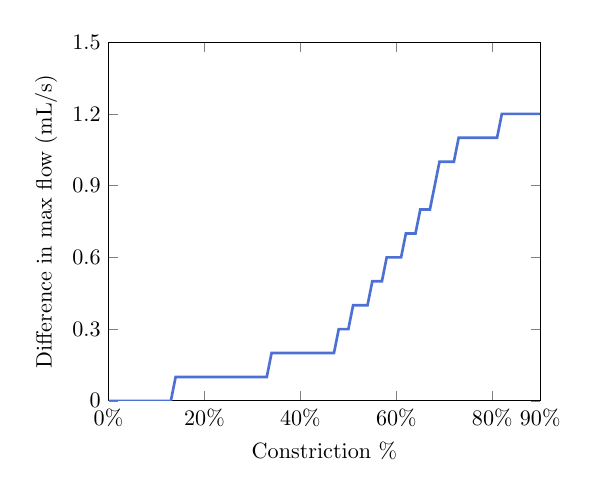
\begin{tikzpicture}[scale=.8]
            % @setfileprefix(data/asymmetric/27e39fe0855e487b61352dea5361a8046716006e/)

\begin{axis}[
    xlabel={Constriction \%},
    xticklabel={$\pgfmathprintnumber{\tick}$\%},
    ylabel={Difference in max flow (mL/s)},
    xmin=0, xmax=90,
    ymin=0, ymax=1.5,
    xtick={0,20,40,60,80,90},
    ytick={0,.3,.6,.9,1.2,1.5},
]

\addplot[color=softblue,style=very thick] coordinates {
    (0,0.0)(1,0.0)(2,0.0)(3,0.0)(4,0.0)(5,0.0)(6,0.0)(7,0.0)(8,0.0)(9,0.0)(10,0.0)(11,0.0)(12,0.0)(13,0.0)(14,0.1)(15,0.1)(16,0.1)(17,0.1)(18,0.1)(19,0.1)(20,0.1)(21,0.1)(22,0.1)(23,0.1)(24,0.1)(25,0.1)(26,0.1)(27,0.1)(28,0.1)(29,0.1)(30,0.1)(31,0.1)(32,0.1)(33,0.1)(34,0.2)(35,0.2)(36,0.2)(37,0.2)(38,0.2)(39,0.2)(40,0.2)(41,0.2)(42,0.2)(43,0.2)(44,0.2)(45,0.2)(46,0.2)(47,0.2)(48,0.3)(49,0.3)(50,0.3)(51,0.4)(52,0.4)(53,0.4)(54,0.4)(55,0.5)(56,0.5)(57,0.5)(58,0.6)(59,0.6)(60,0.6)(61,0.6)(62,0.7)(63,0.7)(64,0.7)(65,0.8)(66,0.8)(67,0.8)(68,0.9)(69,1.0)(70,1.0)(71,1.0)(72,1.0)(73,1.1)(74,1.1)(75,1.1)(76,1.1)(77,1.1)(78,1.1)(79,1.1)(80,1.1)(81,1.1)(82,1.2)(83,1.2)(84,1.2)(85,1.2)(86,1.2)(87,1.2)(88,1.2)(89,1.2)(90,1.2)
    % % @generated(fields='1,2', range=2.., transform='lambda x, y: (x, str(float(y)*1000))', summary-10d-28s-tanh:8.00s-4s-4s.csv)
};

\end{axis}

        \end{tikzpicture}
        \subcaption{Difference in maximum flow}
    \end{subfigure}%
    \begin{subfigure}[t]{0.5\textwidth}
        \centering
        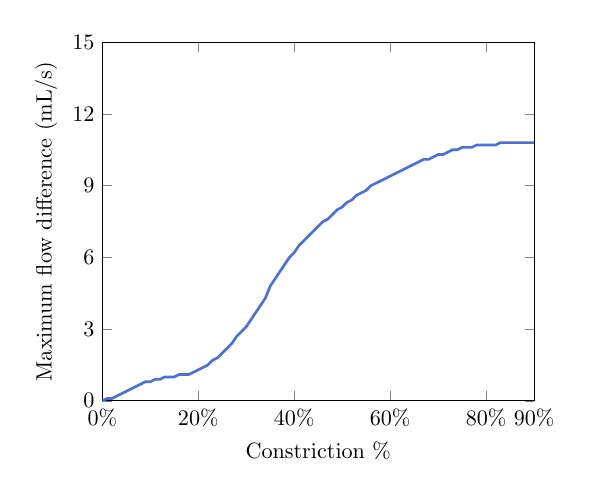
\begin{tikzpicture}[scale=.8]
            % @setfileprefix(data/asymmetric/27e39fe0855e487b61352dea5361a8046716006e/)

\begin{axis}[
    xlabel={Constriction \%},
    xticklabel={$\pgfmathprintnumber{\tick}$\%},
    ylabel={Maximum flow difference (mL/s)},
    xmin=0, xmax=90,
    ymin=0, ymax=15,
    xtick={0,20,40,60,80,90},
    ytick={0,3,6,9,12,15},
]

% weirdly wasn't working, so copy+pasted here :)
\addplot[color=softblue,style=very thick] coordinates {
    (0,0.0)(1,0.1)(2,0.1)(3,0.2)(4,0.3)(5,0.4)(6,0.5)(7,0.6)(8,0.7)(9,0.8)(10,0.8)(11,0.9)(12,0.9)(13,1.0)(14,1.0)(15,1.0)(16,1.1)(17,1.1)(18,1.1)(19,1.2)(20,1.3)(21,1.4)(22,1.5)(23,1.7)(24,1.8)(25,2.0)(26,2.2)(27,2.4)(28,2.7)(29,2.9)(30,3.1)(31,3.4)(32,3.7)(33,4.0)(34,4.3)(35,4.8)(36,5.1000000000000005)(37,5.4)(38,5.7)(39,6.0)(40,6.2)(41,6.5)(42,6.7)(43,6.8999999999999995)(44,7.1000000000000005)(45,7.3)(46,7.5)(47,7.6)(48,7.8)(49,8.0)(50,8.1)(51,8.3)(52,8.4)(53,8.6)(54,8.7)(55,8.8)(56,9.0)(57,9.1)(58,9.2)(59,9.299999999999999)(60,9.4)(61,9.5)(62,9.6)(63,9.700000000000001)(64,9.799999999999999)(65,9.9)(66,10.0)(67,10.1)(68,10.1)(69,10.200000000000001)(70,10.3)(71,10.3)(72,10.4)(73,10.5)(74,10.5)(75,10.6)(76,10.6)(77,10.6)(78,10.7)(79,10.7)(80,10.7)(81,10.7)(82,10.7)(83,10.8)(84,10.8)(85,10.8)(86,10.8)(87,10.8)(88,10.8)(89,10.8)(90,10.8)
    % @generated(fields='1,3', range=2.., transform='lambda x, y: (x, str(float(y)*1000))', summary-10d-28s-tanh:8.00s-4s-4s.csv)
};

\end{axis}

        \end{tikzpicture}
        \subcaption{Maximum difference in flow at the same time}
    \end{subfigure}
    \caption{
        As constriction in the left lung increases, comparisons of the flow in the right lung with a
        right lung from a healthy left lung. \textbf{N.B.}: Units are measured in millilitres; the
        differences are very small.
    }
    \label{fig:asymmetric-flow-diff}
\end{figure}

There is, however, an imperceptibly small difference between the flow from the right lung in this
trial, and one where the left lung remained healthy the entire time: At 50\% constriction in the
left lung, the maximum flow through the right lung is 0.3 mL/s greater than with no
constriction~--~and at one point in time, the difference between the two flows is 8.1 mL/s.

Clearly these are still small, but it is worth quantifying these differences and observing how they
change with constriction; so \autoref{fig:asymmetric-flow-diff} displays both of these metrics. With
a quick look at the two charts, it is clear that even with the most severe constriction on the left
lung, the flow through the right lung barely changes, supporting the initial observations from
\autoref{fig:asymmetric-recovery}.


\newpage
% Ch5-conclusions.tex
%
% vim: set ft=tex:
\section{Conclusions}

\subsection{Summary of key results} \label{sec:summary-of-key-results}

In this paper, we have used recent, established mathematical models to investigate the
characteristics of airflow in the lungs under a variety of conditions. In particular, we've
demonstrated a clear association between maximum acceleration in flow and airway constrict, in a
way that is not as visible in just the maximum speed of flow reached.

From there, we introduce the ``constrict and recover'' pattern, where the airways in an
initially-healthy lung are gradually constricted to a desired level and after a delay, they
gradually return back to the healthy state. The flow characteristics as the constriction level
changes appear \textit{similar} to a composition of the flows from intermediate constriction levels,
and we show the way that this effect is rooted in the basic mechanics of the system, explaining why
this causes the airflow to appear abnormal at certain points.

Extrapolating from this, we find a particular worst-case scenario wherein the quick correction from
one volume to the ``target'' volume for the pleural pressure cauess an extreme spike in the airflow
velocity.

And finally, we show by asymmetric constriction that the primary source of resistance is not coming
from the trachea. This is not \textit{necessarily} incorrect, but it is certainly interesting,
considering that prior studies have shown that the majority of airflow resistance in the lungs comes
from the larger conducting airways. One possible explanation for this is the exact method we were
using for whole lung constriction~--~in practice it \textit{may} be more likely that typical airway
constriction (e.g., from asthma) has a greater proportional effect on the larger airways.

\subsection{Limitations and further work} \label{sec:limitations-and-further-work}

There are of course a number of areas of possible improvement for the our experiments~--~a number of
which have been briefly mentioned already, but they bear repeating. From a purely technical
standpoint, it's certainly possible to obtain more efficient models with a better matrix
factorisation algorithm; GMRES will likely perform much better, but perhaps the most significant
gains in simulation size and speed would come from parallel factorisation.

There are also a number of avenues for improvement in the accuracy of the simulation: An immediate
improvement would be to use models synthesized from lung scans, as in \cite{FoyEtAl2017}. But
particularly as we increase constriction, it is also unreasonable to expect that the pleural
pressure will remain the same~--~a model of pleural pressure that reacts to the lung volume in a
similar way to humans may provide a more accurate result when looking at severe constriction.

\breakpars

Looking forward, there are possible applications of this research outside of this field~--~fast and
efficient simulation provides a key opportunity to use this tool to provide data for data-intensive
applications, like machine learning (in \cite{SuoEtAl2021}, for example, data was gathered from a
physical system where it could have been done by modifying this software).

There are also possibilities within this space. Given the results on maximum flow acceleration,
there may room for new multiple-breath washout indices that are more sensitive to constriction that
is not as severe.


\newpage
\bibliography{ref.bib}{}
\bibliographystyle{abbrvnat}

\newpage

\begin{appendices}
% Appendices.tex
%
% vim: set ft=tex:

% helper derived from https://tex.stackexchange.com/a/252667
\titleformat{\section}{\normalfont\large\bfseries}{Appendix \thesection:}{1em}{}
\section{Extended equations} \label{appendix:equations}

\def\plmin{P_{\text{pl}_{\text{min}}}}
\def\plmax{P_{\text{pl}_{\text{max}}}}
\def\plinit{P_{\text{pl}_{\text{init}}}}

In \autoref{sec:simultaneous-equations}, the function controlling pleural pressure is referenced. It
is defined here, using a minimum $\plmin$, maximum $\plmax$ and initial pressure $\plinit$. The
period is $T$.

\begin{equation}
    P_{\text{pl}}(t_n) = M - A \cos\left(\frac{2\pi}{T} t_n + \cos^{-1}\left( \frac{M - \plinit}{A} \right)\right)
\end{equation}

\noindent where

\begin{align*}
    A &= \frac{\plmax - \plmin}{2}\hspace{1cm}&\text{(amplitude)} \\
    M &= \frac{\plmax + \plmin}{2}\hspace{1cm}&\text{(mean)}
\end{align*}

\noindent This function has the property that~--~if the initial value is not the minimum or maximum
value~--~it is always increasing at $t_n = 0$. If the initial value is the minimum,
$P_{\text{pl}}(t_n)$ is not technically increasing at $t_n = 0$, but it will be at $t_n = \epsilon$.

\end{appendices}

\end{document}
